\documentclass[11pt]{article}

\usepackage[margin=1in]{geometry}
\usepackage{booktabs}
\usepackage{graphicx}
\usepackage{microtype}
\usepackage{amsmath}
\usepackage{hyperref}
\usepackage{xcolor}
\usepackage{enumitem}
\usepackage{natbib}

\hypersetup{
  colorlinks=true,
  linkcolor=blue!55!black,
  citecolor=blue!55!black,
  urlcolor=blue!55!black
}

\title{Fragile Correctness in Long Reasoning Traces:\\
Correct Answers That Disappear Across Seeds}

\author{
  Anonymous Authors\\
  \texttt{logit\_cot\_overthinking}
}

\date{\today}

\begin{document}
\maketitle

\begin{abstract}
Reasoning models often improve as they generate more thinking tokens, but
some trajectories appear to pass through a correct answer and then end
incorrectly. We study this phenomenon using logit-based trajectory probing:
generate a full reasoning trace, slice the trace at token deciles, reinsert
each prefix, and measure the next-token probability assigned to valid
multiple-choice answers. Using \texttt{google/gemma-4-12B-it} on MMLU-Pro and
GPQA Diamond, we find preliminary evidence that these ``lost correctness''
events are not merely noise from long traces. In matched-control reruns across
ten seeds, questions that lost the correct answer at seed 0 lost it again at
46.8\% of attempts in both datasets, compared with 5.2--17.6\% for
final-correct controls and 16.0--18.8\% for stable-wrong controls matched by
category and trace length. Among checkpoints where the model is currently
correct, future loss is predictable from instability features such as prior
answer flips and confidence decline; at the 80\% checkpoint, a grouped
cross-validated classifier reaches AUC 0.817 using instability features,
compared with AUC 0.718 from current confidence alone. We propose a new
hypothesis: some tasks induce \emph{fragile correctness}, a state where the
model has found the correct answer but has not stabilized it. We outline
intervention experiments to test whether early commitment, branching, or
answer-preserving trace policies can turn fragile correctness into reliable
final accuracy.
\end{abstract}

\section{Introduction}

Large language models increasingly solve difficult questions by generating
long reasoning traces before committing to an answer
\citep{wei2022chain,wang2022selfconsistency}. A common expectation is that
additional reasoning should, on average, improve performance: the model has
more opportunity to decompose the problem, retrieve relevant facts, and check
intermediate conclusions. Recent trajectory-probing work supports this
aggregate picture, showing that accuracy and answer commitment often increase
as more reasoning tokens are supplied back to a model \citep{ballon2026probing}.

The aggregate trend, however, leaves an important reliability question open.
What happens when a model is already correct partway through its reasoning,
but later changes away from the correct answer? Such cases are practically
important because they expose a failure mode that is invisible if one only
evaluates final answers. They also matter for deployment: if future loss can
be predicted online, then a system might stop, branch, or intervene before
the final answer degrades.

This draft reports an initial investigation of this phenomenon. We adapt the
three-stage logit trajectory probe of \citet{ballon2026probing} to
\texttt{google/gemma-4-12B-it}. We generate complete thinking traces for
multiple-choice questions, slice the hidden thought content at deciles, and
probe the distribution over answer-letter tokens after each prefix. A
\emph{broad loss} occurs when the correct answer is the probe prediction at
some checkpoint but not at the final checkpoint.

Our initial results suggest that loss is not simply a side effect of long
reasoning or random sampling. Instead, it appears concentrated in a subset of
questions that repeatedly induce unstable trajectories. We call this
\emph{fragile correctness}: a correct intermediate answer state that has not
become robust to further reasoning.

\paragraph{Contributions.}
This draft makes three preliminary contributions:

\begin{enumerate}[leftmargin=*]
  \item We implement a Gemma-specific trajectory-probing pipeline over
  MMLU-Pro \citep{wang2024mmlupro} and GPQA Diamond \citep{rein2023gpqa},
  including answer-letter log-probabilities, trajectory metrics, capped-trace
  extension, and matched reruns.

  \item We introduce a matched-control design for studying lost correctness.
  For each dataset, we select seed-0 loss questions, final-correct controls,
  and stable-wrong controls, matched within category and by seed-0 trace
  length, and rerun each selected question over ten seeds.

  \item We find that seed-0 loss questions are much more likely to lose the
  correct answer again than either control group. We also find that, among
  currently-correct checkpoints, future loss is predictable from instability
  features beyond current confidence.
\end{enumerate}

\section{Trajectory Probing}

We use a logit-based trajectory probe rather than asking the model to
self-report whether it has solved the question. For each question, the model
first generates a complete reasoning trace using thinking-enabled sampling.
We extract the content of Gemma's thought channel, tokenize it, and slice it
at 0\%, 10\%, \ldots, 100\% using token-count ceilings. Each prefix is then
reinserted into the prompt, the thought channel is closed, and the model is
asked for exactly one answer token with sampling disabled. We request raw
log-probabilities for the valid answer-letter token IDs and compute normalized
choice probabilities, non-choice probability mass, predictions, correctness,
final-answer commitment, answer flips, and endpoint trajectory class.

This design follows \citet{ballon2026probing}, with adaptations for
Gemma's thought-channel formatting and the variable answer-choice structure
of MMLU-Pro and GPQA Diamond. All probes are answer-letter probes: for a
question with valid choices $\mathcal{C}$, the predicted answer at checkpoint
$t$ is
\[
  \hat{y}_t = \arg\max_{c \in \mathcal{C}} p_t(c),
\]
where $p_t(c)$ is the one-token probability assigned to answer letter $c$
after reinserting the prefix ending at checkpoint $t$.

\section{Hypothesis: Fragile Correctness}

Our starting observation was that some traces become correct before the end
but finish incorrectly. A tempting explanation is generic overthinking:
longer traces give the model more chances to talk itself out of the right
answer. The matched-control results below point to a sharper hypothesis.

\paragraph{Fragile correctness hypothesis.}
Some questions induce intermediate states where the model has identified the
correct answer but has not stabilized the answer against future reasoning.
These states are characterized by unstable answer trajectories: frequent
answer flips, declining normalized probability on the correct answer, and
language suggestive of repeated reconsideration or re-derivation. Future loss
should therefore recur across seeds for the same question, and should be
predictable from trajectory instability while the model is still currently
correct.

This hypothesis differs from a pure length hypothesis. A pure length
hypothesis predicts that matched questions with similar trace lengths should
show similar loss rates. Fragile correctness predicts that seed-0 loss
questions should remain high-risk even after matching on length and category.

\section{Experimental Design}

\subsection{Source Runs}

We first ran the trajectory probe on a balanced 1,000-question MMLU-Pro sample
and the full 198-question GPQA Diamond split using
\texttt{google/gemma-4-12B-it} \citep{gemma4model}. The model was sampled for
traces with Gemma-recommended settings and probed greedily for one token at
each decile.
Trace generation used a 16,384-token cap. Capped traces were subsequently
continued with an additional 16,384-token budget under a larger 49,152-token
context; traces that still did not naturally close were explicitly
force-closed and retained with a \texttt{forced\_completion} flag.

\subsection{Matched-Control Reruns}

From the source runs, we built matched triplets in each dataset. Each triplet
contains:

\begin{itemize}[leftmargin=*]
  \item a seed-0 \textbf{loss} question: correct at some checkpoint but wrong
  at the final checkpoint;
  \item a seed-0 \textbf{final-correct} control: correct at the final
  checkpoint; and
  \item a seed-0 \textbf{stable-wrong} control: never correct across the
  probed checkpoints.
\end{itemize}

Controls are matched within dataset and category to the nearest seed-0 trace
length. Each dataset contributes 25 triplets, so the rerun experiment contains
150 unique questions: 75 from MMLU-Pro and 75 from GPQA Diamond. We rerun
every question for seeds 0 through 9, yielding 1,500 full traces and 16,500
decile probe rows before extension. The raw matched-control run produced 282
capped traces. All capped traces were extended and re-probed, leaving zero
remaining truncation. Twenty-six traces required forced closure: 24 in GPQA
Diamond and 2 in MMLU-Pro.

\subsection{Predicting Future Loss}

We also ask whether future loss is predictable while the model is currently
correct. We construct one supervised row for each checkpoint in
$\{10,20,\ldots,90\}$ where the current probe prediction is correct. The
target is whether the final checkpoint is incorrect. We evaluate logistic
models with five-fold cross-validation grouped by question, so different
seeds of the same question never appear in both train and test folds.

We compare four feature sets:

\begin{description}[leftmargin=*]
  \item[Confidence.] Current normalized probability assigned to the correct
  answer.
  \item[Instability.] Confidence plus flips so far, confidence decline from
  the peak, time since first correct, and current stable-correct streak.
  \item[Instability + length.] Instability plus final trace length. This is
  an oracle feature and is included only as a diagnostic.
  \item[Full prefix.] Instability plus length and simple prefix-language
  features for self-correction, simulated retrieval, and repetition.
\end{description}

\section{Initial Results}

\subsection{Loss Recurs Across Seeds}

Table~\ref{tab:recurrence} shows the matched-control recurrence results.
Seed-0 loss questions lose the correct answer much more often than either
matched control cohort. This is true in both datasets. In GPQA Diamond, the
loss cohort has a 46.8\% broad-loss rate across reruns, compared with 17.6\%
for final-correct controls and 16.0\% for stable-wrong controls. In MMLU-Pro,
the loss cohort again has a 46.8\% broad-loss rate, compared with 5.2\% and
18.8\% for the two controls.

\begin{table}[t]
  \centering
  \small
  \begin{tabular}{llrrrr}
    \toprule
    Dataset & Seed-0 cohort & Attempts & Broad losses & Rate & Final acc. \\
    \midrule
    GPQA Diamond & final correct & 250 & 44 & 17.6\% & 78.8\% \\
    GPQA Diamond & loss & 250 & 117 & 46.8\% & 43.6\% \\
    GPQA Diamond & stable wrong & 250 & 40 & 16.0\% & 21.6\% \\
    MMLU-Pro & final correct & 250 & 13 & 5.2\% & 86.4\% \\
    MMLU-Pro & loss & 250 & 117 & 46.8\% & 45.6\% \\
    MMLU-Pro & stable wrong & 250 & 47 & 18.8\% & 15.2\% \\
    \bottomrule
  \end{tabular}
  \caption{Matched-control rerun results. A broad loss means the correct
  answer is predicted at some checkpoint but not at the final checkpoint.}
  \label{tab:recurrence}
\end{table}

Bootstrap risk differences over the 25 matched triplets are all positive.
For GPQA Diamond, the loss cohort exceeds final-correct controls by
29.2 percentage points (95\% CI: 15.6 to 43.2) and stable-wrong controls by
30.8 points (95\% CI: 16.8 to 44.8). For MMLU-Pro, the corresponding risk
differences are 41.6 points (95\% CI: 31.2 to 52.4) and 28.0 points
(95\% CI: 15.2 to 40.8).

\begin{figure}[t]
  \centering
  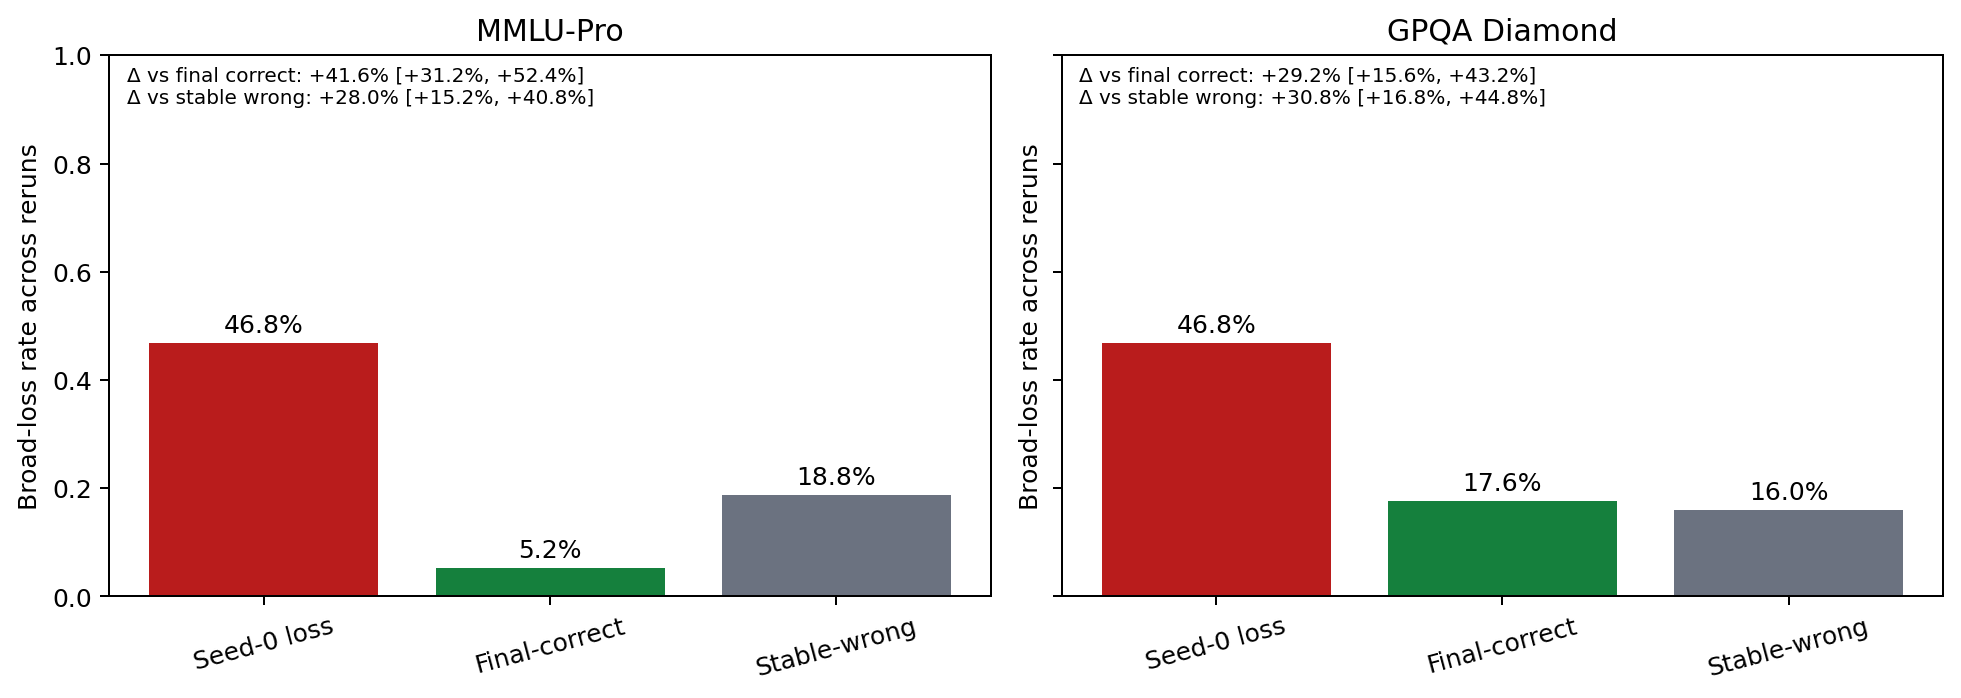
\includegraphics[width=0.95\linewidth]{figures/cohort_loss_rates.png}
  \caption{Broad-loss recurrence by seed-0 cohort. Loss questions show much
  higher recurrence than category- and trace-length-matched controls.}
  \label{fig:cohort-loss}
\end{figure}

\subsection{Instability Predicts Future Loss}

Table~\ref{tab:auc} summarizes future-loss prediction at 50\% and 80\%
checkpoints. At 50\%, confidence alone is already informative in the combined
sample (AUC 0.732), but instability features are comparable. By 80\%, the
instability features become much stronger: combined AUC rises from 0.718 with
confidence alone to 0.817 with trajectory-instability features. The pattern
is strongest in MMLU-Pro, where 80\% AUC rises from 0.697 to 0.853, and is
also present in GPQA Diamond, where 80\% AUC rises from 0.585 to 0.755.

\begin{table}[t]
  \centering
  \small
  \begin{tabular}{llrrrr}
    \toprule
    Dataset & Checkpoint & Confidence & Instability & + length & + prefix \\
    \midrule
    Combined & 50\% & 0.732 & 0.731 & 0.764 & 0.755 \\
    Combined & 80\% & 0.718 & 0.817 & 0.810 & 0.812 \\
    MMLU-Pro & 50\% & 0.667 & 0.698 & 0.701 & 0.678 \\
    MMLU-Pro & 80\% & 0.697 & 0.853 & 0.857 & 0.851 \\
    GPQA Diamond & 50\% & 0.670 & 0.731 & 0.732 & 0.731 \\
    GPQA Diamond & 80\% & 0.585 & 0.755 & 0.748 & 0.762 \\
    \bottomrule
  \end{tabular}
  \caption{Question-grouped cross-validated AUC for predicting future loss
  from checkpoints where the model is currently correct.}
  \label{tab:auc}
\end{table}

\begin{figure}[t]
  \centering
  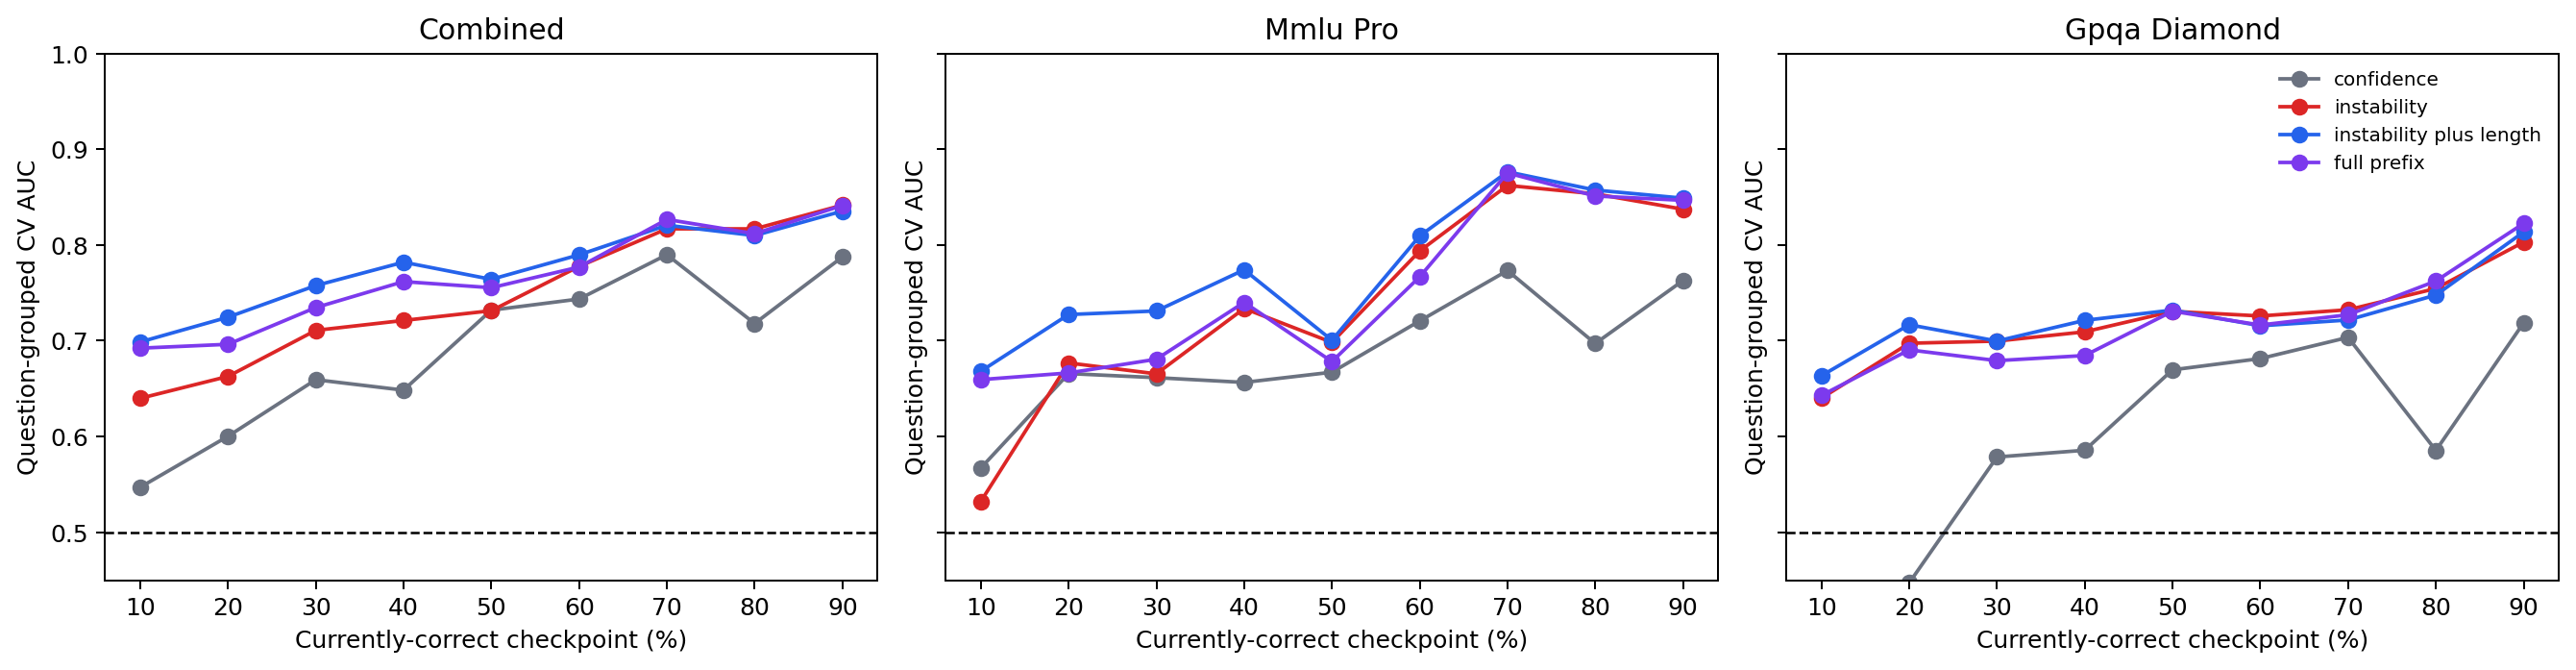
\includegraphics[width=0.95\linewidth]{figures/predictive_auc_by_decile.png}
  \caption{Future-loss prediction across currently-correct checkpoints. Late
  instability features are more informative than current confidence alone.}
  \label{fig:auc}
\end{figure}

\subsection{Late-Stage Signals}

At the 80\% checkpoint in the combined full-prefix model, the strongest
positive standardized coefficients are normalized confidence decline
(+0.334), prefix repetition score (+0.308), prefix self-correction (+0.272),
and flips so far (+0.203). These features are associations, not causal
effects, but they are consistent with the fragile-correctness hypothesis:
future loss is linked to unstable answer dynamics rather than merely to a
low current probability on the correct answer.

\begin{figure}[t]
  \centering
  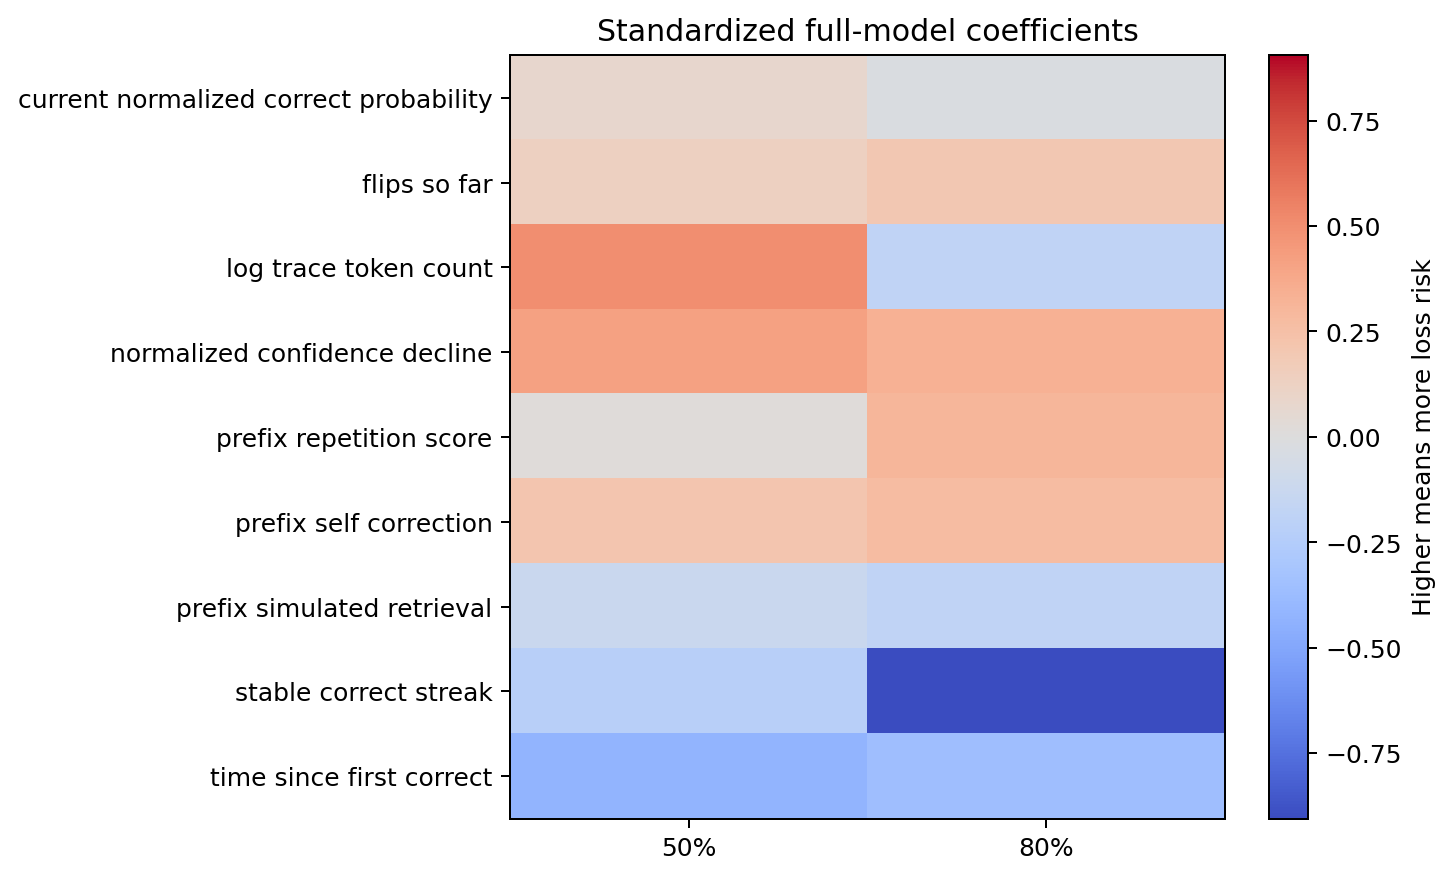
\includegraphics[width=0.75\linewidth]{figures/feature_coefficients.png}
  \caption{Standardized coefficients from the full-prefix predictor for the
  combined dataset at 50\% and 80\% checkpoints.}
  \label{fig:coefficients}
\end{figure}

\subsection{Forced-Completion Sensitivity}

The extension step force-closed 26 traces that still did not naturally finish
after an additional 16,384-token continuation budget. Forced completions do
not explain the central recurrence effect. In the matched-control analysis,
the loss cohorts have zero forced completions. Excluding forced completions
from the controls leaves the broad-loss rates nearly unchanged: GPQA
final-correct controls move from 17.6\% to 17.4\%, GPQA stable-wrong controls
from 16.0\% to 16.6\%, and MMLU-Pro stable-wrong controls from 18.8\% to
19.0\%.

\section{Discussion}

The most important observation is that lost correctness appears to be
question-specific and repeatable. If loss were mostly generic overthinking,
then category- and length-matched controls should show similar loss rates.
Instead, seed-0 loss questions recur as losses at much higher rates. This
suggests that the question itself, or the model's representation of that
question, induces a fragile reasoning trajectory.

The predictor results sharpen this interpretation. Current confidence alone
is informative but incomplete. Late in the trace, instability features such
as answer flips and confidence decline are better predictors of future loss.
This suggests that an online monitor could detect when a correct answer has
not stabilized and trigger a policy intervention.

The results do not show that reasoning traces are bad on average. In fact,
the original trajectory-probing paper and our own aggregate curves are
compatible with the usual result that more reasoning often helps. The claim
is narrower: for a subset of questions, the model can enter a correct but
unstable state, and continued generation can destroy rather than consolidate
that state.

\section{Next Experiments}

The current evidence is associative. The next experiments should test whether
fragile correctness can be converted into final accuracy by intervention.

\paragraph{1. Early-commitment intervention.}
For every checkpoint where the probe is correct, stop the model and emit an
answer immediately. First evaluate an oracle policy that stops at the first
correct checkpoint to estimate the maximum recoverable accuracy. Then replace
the oracle with practical policies: stop when normalized correct probability
exceeds a threshold, stop when confidence is high and stable for two
checkpoints, or stop when instability features predict high future-loss risk.
The key outcome is whether these policies improve final accuracy on loss
questions without hurting final-correct controls.

\paragraph{2. Branching after fragile-correct checkpoints.}
When the model is currently correct but predicted to be fragile, branch into
several answer-only or short-verification continuations. Compare standard
continuation, answer-only commitment, and verification prompts that ask the
model to preserve or challenge its current answer. If branching rescues loss
cases, it would provide stronger evidence that the correct state is present
but unstable.

\paragraph{3. Counterfactual continuation from matched prefixes.}
Take prefixes from loss and control questions at matched deciles and continue
them under multiple seeds. This isolates whether the risky state is already
encoded in the prefix. A strong result would show that prefixes with similar
current confidence have different loss probabilities depending on their
prior instability history.

\paragraph{4. Larger and cross-model replication.}
Scale the matched-control reruns beyond 25 triplets per dataset, then repeat
on larger Gemma, Qwen, and other reasoning models. The central question is
whether fragile correctness is a general property of reasoning models or a
Gemma-specific failure mode.

\paragraph{5. Online predictor calibration.}
Train predictors on one dataset and evaluate on the other, and train on one
set of questions while evaluating on held-out categories. Report calibration
curves, precision-recall tradeoffs, and the cost of false early stops. This
is necessary before using the detector as a deployment policy.

\paragraph{6. Qualitative and semantic analysis of lost cases.}
Annotate high-risk traces for mechanisms: competing plausible answers,
retrieval errors, late contradiction, arithmetic drift, option misreading,
and repeated self-correction loops. Pair this with automated prefix-language
features to determine whether the linguistic signals are proxies for
specific reasoning failures.

\section{Limitations}

This is an initial result. The matched-control experiment uses 25 triplets
per dataset, so confidence intervals should be treated as preliminary. The
trajectory probe measures the distribution induced by reinserting a trace
prefix; it does not prove that the hidden trace is a faithful explanation of
the model's internal computation. The length feature in the predictor is an
oracle feature because the final trace length is not known to an online
system. Finally, forced closure is a practical necessity for runaway traces,
though the main recurrence effect is not driven by forced completions.

\section{Conclusion}

These initial experiments support a pivot from a generic overthinking
hypothesis to a fragile-correctness hypothesis. Some questions repeatedly
lead the model to a correct intermediate answer that is not stable under
continued reasoning. This failure mode is detectable before the final answer:
late answer flips, confidence decline, repetition, and self-correction are
associated with future loss. The next step is to move from diagnosis to
intervention, testing whether early commitment and branching policies can
recover answers that the model already found but would otherwise lose.

\bibliographystyle{plainnat}
\bibliography{references}

\end{document}
